\documentclass[10pt,conference,compsocconf]{IEEEtran}

\usepackage{hyperref}
\usepackage{graphicx}	% For figure environment

\begin{document}
\title{Earthquake Detection from Seismological Data}

\author{
  Lucien Michaël Iseli, Florian Maxime Charles Ravasi and Jules Eliot Gottraux\\
  \textit{Master of Data Science, EPFL, Switzerland}
}

\maketitle
\section{Introduction}
In seismology, the detection of earthquakes is a pretty active research. The detection of severe earthquake, those that make your house tremble and are actually dangerous, is not a particularly tricky task but when talking about earthquakes of small magnitude that's a different story. In fact, as of today the detection and classification of earthquakes is still done by hand by specialists. That is they manually inspect the measurements taken by sensors to produce the catalogs, the tables containing the earthquakes's informations. This process is error-prone and tedious, this is why we try to address this issue in this project. We'll use data from sensors that capture the vibration present in the earth, the same data that specialists in detection use, to create a machine learning model able to detect if an earthquake has happened. Most of the work we will present will be prior to the creation and optimization of the machine learning algorithm. That is we spent most of our time preparing the data and doing featuring engineering. As we will see, this task revealed to be very difficult and one would need more time and substantial expertise to obtain satisfying performances for small earthquake detection. However by simplifying the task we managed to get acceptable result. In fact this work is inspired by a research \cite{ConvNetPaper} conducted by three researchers, they worked hard to achieve that using neural networks and clever memory management.

\section{Dataset Characteristics}
We get our data using the ObsPy library \cite{obspy}. ObsPy grants us access to stations, which have sensors that record the seismological activity over time on different channels. Those sensors constantly record  the vibration of the earth at their location. This include seismic waves which are the waves of energy released when a seism occur nearby. This data is thus one dimensional and filled with noise as it is a completely raw measure, it is a giant time series containing the amplitude of waves captured by the sensor. It has the information of the seism and earthquake but this information is aggregated with all the vibration happening near the sensor. The goal will be to create, from this time series, meaningful features for the model containing sufficient information to classify a certain window of time. We'll thus fix the duration of a time window, for example one minute, then compute features on this time window and feed these features to the machine learning model. We also compute the fourier transform of the time window because an earthquake normally has a lot of different frequencies including the high ones. We heuristically noticed that in the fourier transforms low frequencies were always present whether it was noise or an earthquake. Therefore, in order to characterise the earthquakes we for example take the mean and the standard deviation starting from a threshold.

\begin{figure}[h]
  \centering
	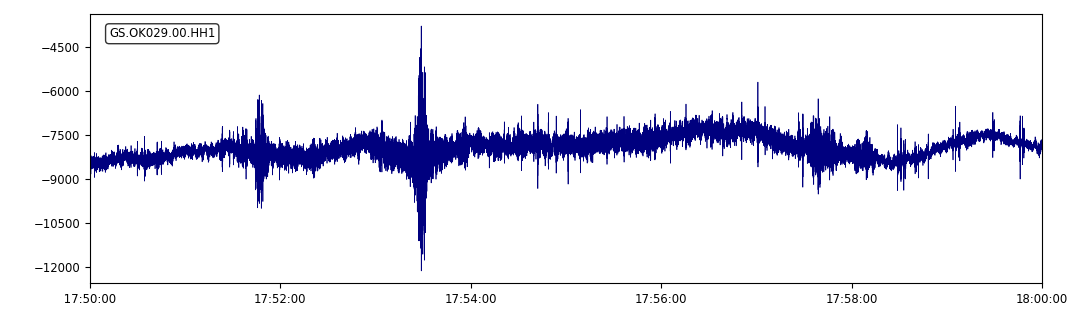
\includegraphics[width=\columnwidth]{10min-example-2018-06-30T17:50_1.png}
  \caption{$10$ minute of data example, no earthquake}
	\label{fig:10min-example}
\end{figure}

So the basis for the features is this time series, for the labels we use a hand-made catalog of earthquake that contains, among other properties, the location, magnitude and time of the earthquake.

Before diving into the machine learning model construction, we have to take care of several difficulties inherent in the dataset.\newline
First the data collection, after having chosen the location, station and channel from which we want to get the time series we have to download it and store that to a usable format for the next steps. The frequency of the sensors is $100$ data point per second, so the amount of data increases quite quickly. Then, the data has holes in it, since it is sometimes missing for some period. Those holes are not regular and unpredictable, so we have to take care of them with caution.

\begin{figure}[h]
  \centering
	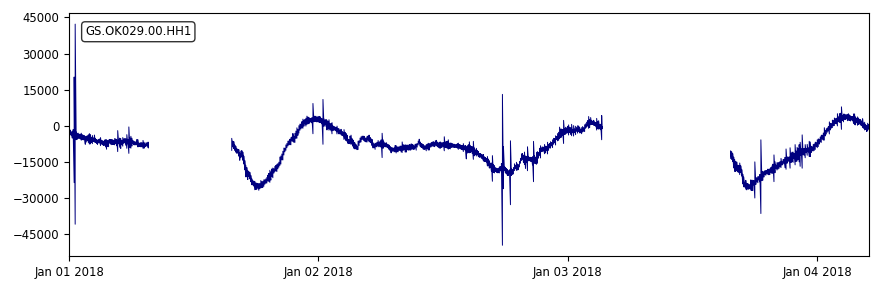
\includegraphics[width=\columnwidth]{hole_example.png}
  \caption{Example of missing values in the dataset}
	\label{fig:10min-example}
\end{figure}

We already mentioned that the data obtained from ObsPy is very noisy, we want to emphasize this and as we will see in examples, some earthquakes and non-earthquakes are undistinguishable for the untrained eye. The catalog is noisy in a sense as well, since the time series are parsed by humans and thus some earthquakes are missed and as the magnitude decreases the number of missed earthquake increases, being the majority for small magnitudes. Another difficulty in the catalog is the delay that is induced by the difference of location between the detection of the earthquake and the location of our station. All the catalog has to be calibrated to ensure that the time of the earthquake corresponds to a peak in our time series. However, the speed of propagation of an earthquake isn't constant. The so-called p-waves' speed of an earthquake varies quite a bit, depending on the rocks it travels through for example. This implies that it is impossible to label perfectly with an automatically method such as ours.\\
To better see what characterise an earthquake we show three examples, one of an obvious and two more difficult to detect earthquakes.

\begin{figure}[h]
  \centering
	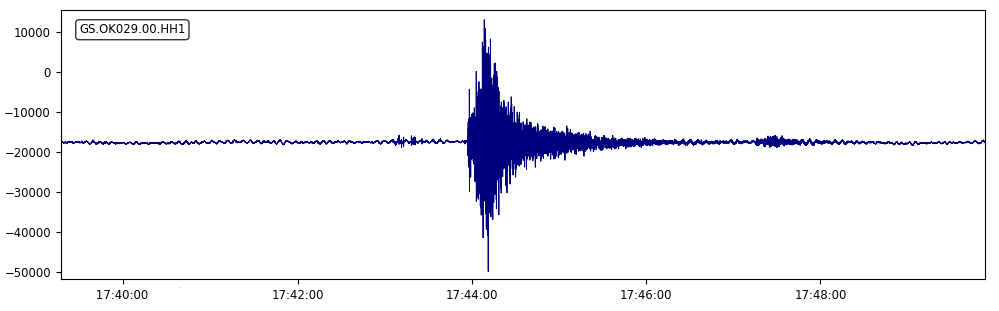
\includegraphics[width=\columnwidth]{fat-earthquake-example.png}
  \caption{Obvious earthquake example, magnitude of $3.5$}
	\label{fig:obvious}
\end{figure}

\begin{figure}[h]
  \centering
	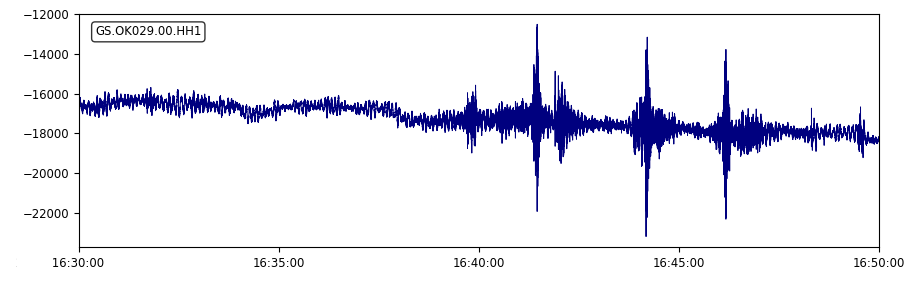
\includegraphics[width=\columnwidth]{multiple-peaks-example.png}
  \caption{Example of earthquake with multiple peaks, magnitude of $2.1$}
	\label{fig:multiplepeaks}
\end{figure}
\begin{figure}[h]
  \centering
	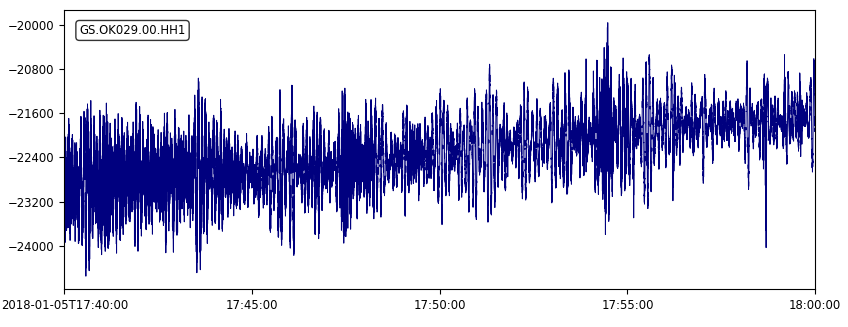
\includegraphics[width=\columnwidth]{constant-variation-example.png}
  \caption{Example of earthquake with constant variation, magnitude of $2.2$}
	\label{fig:constanteq}
\end{figure}

We can see what characterise the easy part of the earthquake in figure \ref{fig:obvious}: A big step at first followed by a slower decrease. During this period, a great amount of different frequencies, including high frequencies are present. The first one is a good example of the discretization problem explained in section \ref{section:labeling}. It is very difficult to determine which of these peaks is part of the earthquake. The see that it is important to keep in mind that they range over more than $5$ minutes. This is big as taking a window of several minutes will most likely not be optimal. The last one shows one of many example of an earthquake that is really difficult to detect. It is not at all the worst, this one has a magnitude of $2.2$ so you can imagine how difficult it is to detect earthquake several times less powerful. These less detectable earthquake are not rare,ones with a magnitudes of less than $1.5$ composes a quarter of our dataset if we take time windows of $1$ minute

\section{Data pre-processing}
We first have to correct the anomalies in the data: the delay induced by the physical distance separating our sensors and the seisms' location and the temporal holes.\newline

First of all, for the missing data, we take care of that when loading it. Whenever a time series has is missing a chunk of its curve, we interpolate it with gaussian noise. This way, it will just be considered as a moment where nothing interesting happened and thus should not worsen the performance as it is quite representative to most of the dataset where no earthquake has happened.

Moreover, as aformentioned, the station we choose records activity and label it with the current time which does not correspond to the exact time at which the earthquake happened according to the catalog we use. Therefore we convert latitude, longitude and elevation to a cartesian coordinate system in order to compute the distance easily. We do this using ECEF coordinates\cite{ECEFPaper}\\
Now that we have the distance, we manually find the start time of some earthquake and see the time difference. With a few time differences and distances we computed the average speed of propagation of earthquake/p-waves and got $5676.611\frac{m}{s}$ which is very close to what they found in \cite{PWavePaper}. We use that measure in order to automatically label the data. We show an example of the delay we add in figure \ref{fig:timediff}. Here, and it is not the furthest earthquake, the delay is already of $10$ seconds which is significant for a time window a one minute.

\begin{figure}[h]
  \centering
	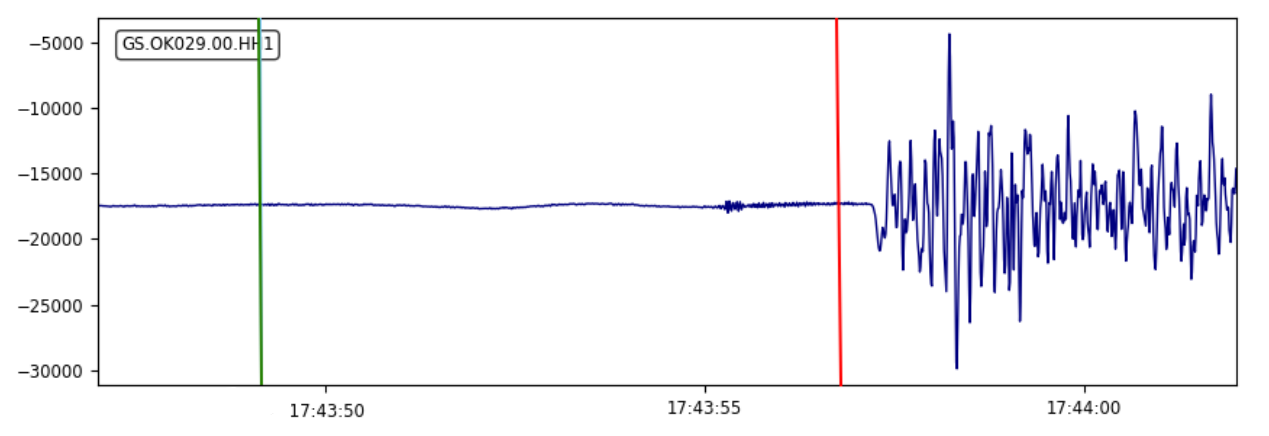
\includegraphics[width=\columnwidth]{time-diff.png}
  \caption{Delay of catalog in green, re-calibrated in red}
	\label{fig:timediff}
\end{figure}


\section{Labeling of the Data}
\label{section:labeling}
Since the dataset lives in a continuous space, we have to discretize it. We have to choose time windows that will be classified as earthquake or not earthquake. The choice of the length of the time window is crucial and it is hard to predict what would be a good choice. Also, that gives rise to a fundamental question for the creation of the labels: when does an earthquake end? It is possible, in fact rather probable depending on the length of the discretization process, that an earthquake spans over multiple time windows thus knowing the duration of the earthquake would permit to overcome this issue. This is important, because not being able to accurately and correctly label our data will of course be disastrous for the machine learning model. Unfortunately, the duration of an earthquake is an open question in geology, the only option simple enough is to label as earthquake only the window that contains the moment of an earthquake.\\
The problem with this approach is illustrated in figure \ref{fig:problem-discretization}. In the catalog the earthquake starts at $T_1$ and we can see that the earthquake indeed triggers a big instant augmentation in the variation of the amplitude, that is typical to the earthquakes that are quite easy to classify. The problem here is that when discretizing the time series in windows, we will likely not have a window starting at $T_1$. Let's say that our partitioning gives a time window that ends at $T_2$. Therefore, we would label the time window containing the start of the earthquake, i.e $T_1$, as an earthquake and hence the one starting at $T_2$ as noise. However, the latter is the one containing most of the earthquake. This labeling is incorrect, we want time windows with such patterns labeled as earthquake because the features have been created to emphasize precisely this kind of pattern. So if the second time window is incorrectly labeled, the negative impact on the algorithm's parameter will be very high. The same problem exists for the testing phase, where for each earthquake the adjacent time windows have a high chance of being mislabeled.

\begin{figure}[h]
  \centering
	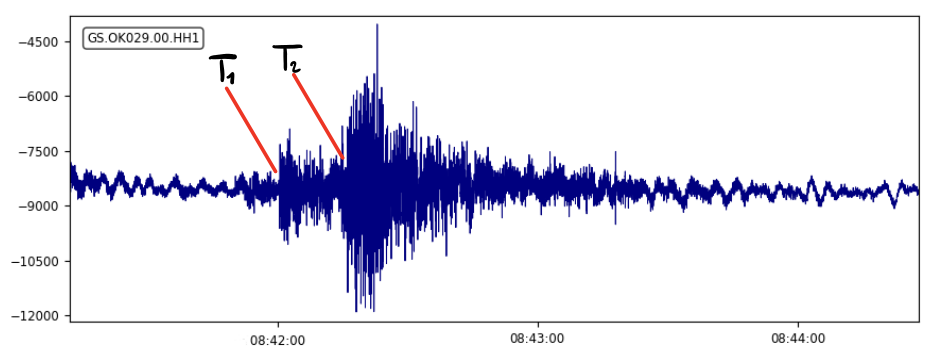
\includegraphics[width=\columnwidth]{problem-time-window-labeling.png}
  \caption{Illustration of the problem of time window labeling}
	\label{fig:problem-discretization}
\end{figure}

\section{Feature Creation}
From that seismic waves we have to choose what processing and transformations will have to be done to be able to feed the machine learning algorithm. We have two main options: leave it as it is and opt for an algorithm such as convolutional neural networks, the approach they took in ConvNetQuake (the paper \cite{ConvNetPaper} that inspired this project), or perform some feature engineering by hand to be able to use some more standard algorithm, which is the approach we chose. So, rather than having a gigantic input dimension we choose to compress it in a smart way, creating meaningful features for the algorithm. For instance, if we took a time window of $10$ seconds, this compression is on the order of $100$ if we create ten features. This permits to accelerate the training process and thus allow to span more time or take more channel.\newline

There are a few characteristics inherent to earthquakes that we try to capture through our features: they have high frequencies, high amplitudes, quick acceleration and a lot of different frequencies. We begin by adding simple measures that directly come to mind:\newline
\begin{itemize}
	\item{Standard deviation of the signal}
	\item{Maximum and minimum of the signal}
	\item{Maximum difference between two adjacent points}
	\item{Maximum and minimum of the shifted signal, shifted meaning the we substract the mean}
	\item{Number of points that are above half of the maximum of the shifted signal, which corresponds to the number of points with high values}
	\item{Number of points that are below half of the minimum of the shifted signal, which corresponds to the number of points with low values}
\end{itemize}

Those features are very simple and may not add much information useful to the model. However we think that the information they add is still positive for what we want to model, the standard deviation, the maximums and the minimums informs us about how variable and powerful is the signal. Earthquakes tends to span much more amplitude and be more unpredictable, hence the standard deviation. The last two features could be useful to prevent false positive.. Indeed, if a noise jump to some high amplitude, it will most likely not have a lot of values extreme values. Hence, if a period containing noise span a lot of amplitude, those measures can help counter this.\\
Now for the main features, the first one capture the speed of variability of the signal, the power of the vibration ina a sense. We compute the number of time that an abrupt change appear in the signal. The second one is a weighted
between adjacent point weighted by the quiteness of the signal before this moment. That way if a peak appear after some quiet period it will capture that, typicall such as in the figure \ref{fig:obvious}. We also compute the fourier transform of the time window because an earthquake normally has a lot of different frequencies including the high ones. We heuristically noticed that in the fourier transforms low frequencies were always present whether it was noise or an earthquake. Therefore, in order to characterise the earthquakes we for example take the mean and the standard deviation starting from a threshold.

\section{Model Selection}
We opted for KNN and RandomForest and describe here our approach with both of them. The problem is that we either tend to have a good precision but low recall or vice-versa, so as shown on the plot below the best F-score we get for both algorithms is quite low. Our training set comprises approximately five months of time windows with $0.45\%$ of earthquakes (the majority being small ones), whereas the test is about one month with $0.46\%$ of earthquakes. It represents $861$ earthquakes for the training set and $214$ for the test set. There are a few parameters that we tweak in order to get better results. Concerning KNN there are two parameters, we change the number of neighbours and we try to compensate the imbalance of the classes by duplicating the earthquake datapoints. Regarding the RandomForest there are three parameters that have a positive influence on our model: the depth of the tree, the number of trees and the weighting of the classes.

\begin{center}
 \begin{tabular}{||c c c||}
 \hline
 Measure & Random Forest & KNN \\ [0.5ex]
 \hline\hline
 Accuracy & 0.97 & 0.99 \\
 \hline
 Precision & 0.06 & 0.098 \\
 \hline
 Recall & 0.38 & 0.08 \\
 \hline
 F1-score & 0.1 & 0.08 \\ [1ex]
 \hline
\end{tabular}
\end{center}

Since little earthquakes do not seem to really trigger our features, we try to simplify our model taking only earthquakes that have at least 2 of magnitude. Here it represents $614$ earthquake for the training set and $138$ for the test set.

\begin{center}
 \begin{tabular}{||c c||}
 \hline
 Measure & Random Forest \\ [0.5ex]
 \hline\hline
 Accuracy & 0.99 \\
 \hline
 Precision & 0.23 \\
 \hline
 Recall & 0.25 \\
 \hline
 F1-score & 0.24 \\ [1ex]
 \hline
\end{tabular}
\end{center}

We see that we get a far better results. So we lost a few earthquakes but really improved our score. Let's see if we can improve it even more taking earthquakes that have at least three of magnitude. Here the training set contains $57$ earthquakes and the test set $6$ of them.

\begin{center}
 \begin{tabular}{||c c||}
 \hline
 Measure & Random Forest \\ [0.5ex]
 \hline\hline
 Accuracy & 1 \\
 \hline
 Precision & 1 \\
 \hline
 Recall & 0.33 \\
 \hline
 F1-score & 0.5 \\ [1ex]
 \hline
\end{tabular}
\end{center}

The F1-score we get is even better than last time, but our recall is still quite low. We see than the magnitude requirement seems to simplify our model enough so that we can almost get a reasonable score. The problem is that the trade-off with the number of earthquakes in our test and training set is really present. Indeed, there are only a few earthquakes left and thus the variance of the result is higher. Indeed, the results we show here represent the best we can get and the higher the magnitude the less the number of earthquakes and thus the higher the variance of the F1-score we get. In order to have a high recall, we can make the weights bigger but the problem is that we get a very low precision in that case.


\section{Conclusion}
That project did not seem hard at first, but we went through many difficulties. First, we had to manually solve the location dependency which is imprecise given that the speed of propagation is variable. Secondly, earthquakes in our data do not always trigger features we expect to characterise them since signals from stations are very noisy. Additionally, automatically splitting the original time series yields chunks that can be mislabled because we only know the start of a seism and since our dataset has a strong uneven proportion of earthquake time windows compared to noisy ones, things can quickly go awry. Then, the feature engineering was not trivial and it took a great amount of time to come up with good approaches that capture the essence of earthquakes.\newline
Thus, after all the pre-processing and feature engineering we did not have that much time left to devote to the training and the model choosing. We did not manage to train a good model for the following reasons: our features did not activate perfectly, our labels were hugely imbalanced and windows were often mislabled. Our first goal was to train a model that detects any earthquake whatever their magnitude. However, small earthquakes are too hard to detect, partly because of the noise, so we decided to focus on those whose magnitude is more than $3$ on the Richter scale. Labeling those earthquake yield better results, going from an almost inexistent F-score to $0.45$, which gives us confidence in our approach.\newline


\section{Further improvements}
There are a few things that we could improve in order to have a better model. The first one is simply to compute better features. Indeed, with better knowledge in geology, and more precisely seismic waves, one could come up with features that captures more how earthquakes' signal behave. Secondly, one could try to come up with a better way to choose time windows that could try to take into account when a seism starts so that it does includes at least a certain percentage of what comes after. Then, in order to have more diversity in our dataset, we could have made use of more than one station; it could have helped with some anomalies that may occur on stations. The more stations we take the less likey we are that they suffer from the same anomalies at the same time; however this greatly increases data size. Detecting low-magnitude earthquakes is a very difficult task, even for experts, but there aren't enough high-magnitude earthquakes to teach the model anything. Indeed, Oklahoma doesn't have a lot of noticeable earthquakes, thus choosing another location could have helped to have a model that is able to detect big earthquakes (big meaning noticeable for a human). To better clean the data we could have also computed the p-wave speed in a more involved manner; we could have for example used ground stucture data to better approximate the speedi, thus having a speed that is dependent on the earthquake location. This could have helped since for the majority of earthquakes our greedy approach works very well but some earthquakes's times are still not perfect. Given the imbalancement of the data, we could have tried to undersample it, helping the algorithm to more adapt its parameter from the earthquake class. We weight the loss function in the algorithm but that can be a better way of handling this imbalance.

\begin{thebibliography}{9}
\bibitem{ConvNetPaper}
Convolutional neural network for earthquake detection and location, 14 February 2018. \\\texttt{https://advances.sciencemag.org/content/4/2/e1700578}
\bibitem{obspy}
ObsPy: python library to collect seismological data.
\\\texttt{https://docs.obspy.org/}
\bibitem{ECEFPaper}
J. Zhu, (1994),  Conversion of Earth-centered Earth-fixed coordinates to geodetic coordinates. \\\texttt{https://ieeexplore.ieee.org/abstract/document/303772/}
\bibitem{PWavePaper}
Guy T. Kuster and M. Nafi Toksöz, (1974), "Velocity and Attenuation of Seismic Waves in two‐phase Media: Part I. Theoretical Formulations," geophysics 39: 587-606. \\\texttt{https://library.seg.org/doi/abs/10.1190/1.1440450}
\end{thebibliography}

\end{document}

